\begin{figure}
    \centering
    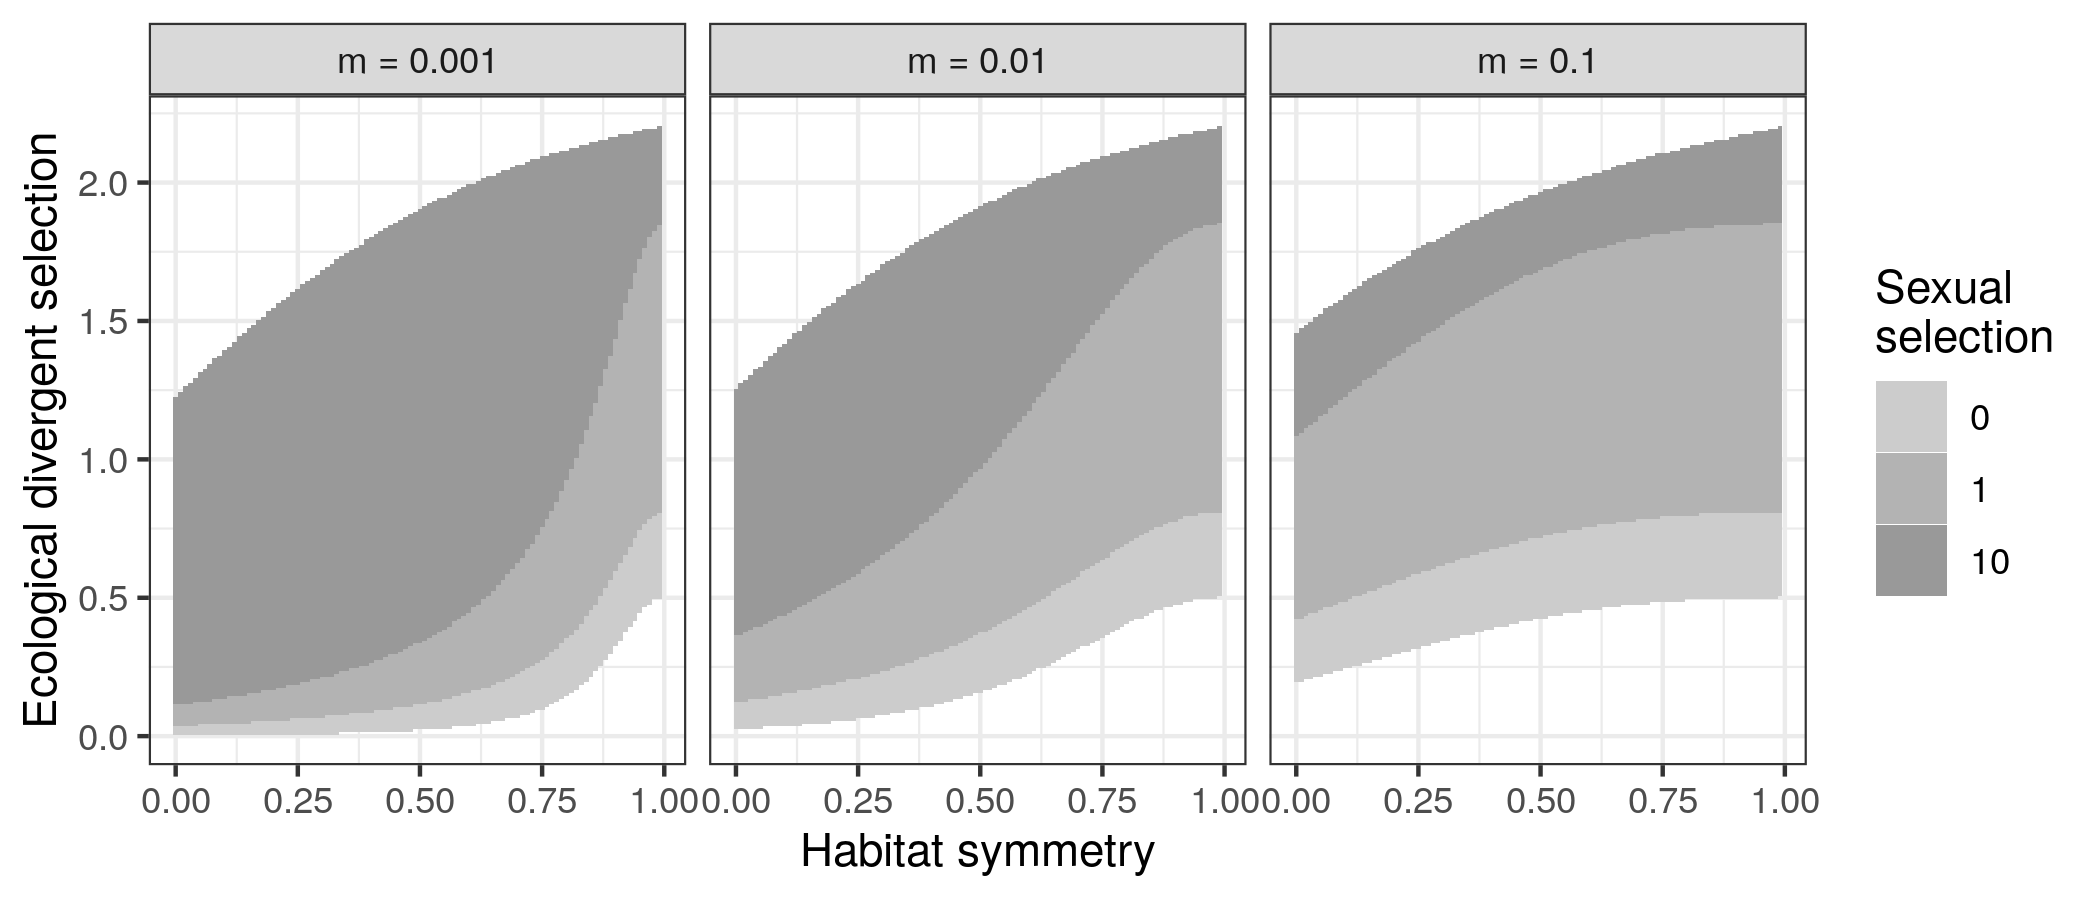
\includegraphics[width=\textwidth]{figures/branching_points}
    \caption{Branching throughout parameter space for three values of the dispersal rate $m$. Sexual selection increases the stability of evolutionary equilibria and therefore turns branching points into stable strategies. Shades of grey indicate the highest tested level $\alpha$ of sexual selection at which branching still occurs.}
    \label{fig:adaptive_dynamics}
\end{figure}


\begin{figure}
    \centering
    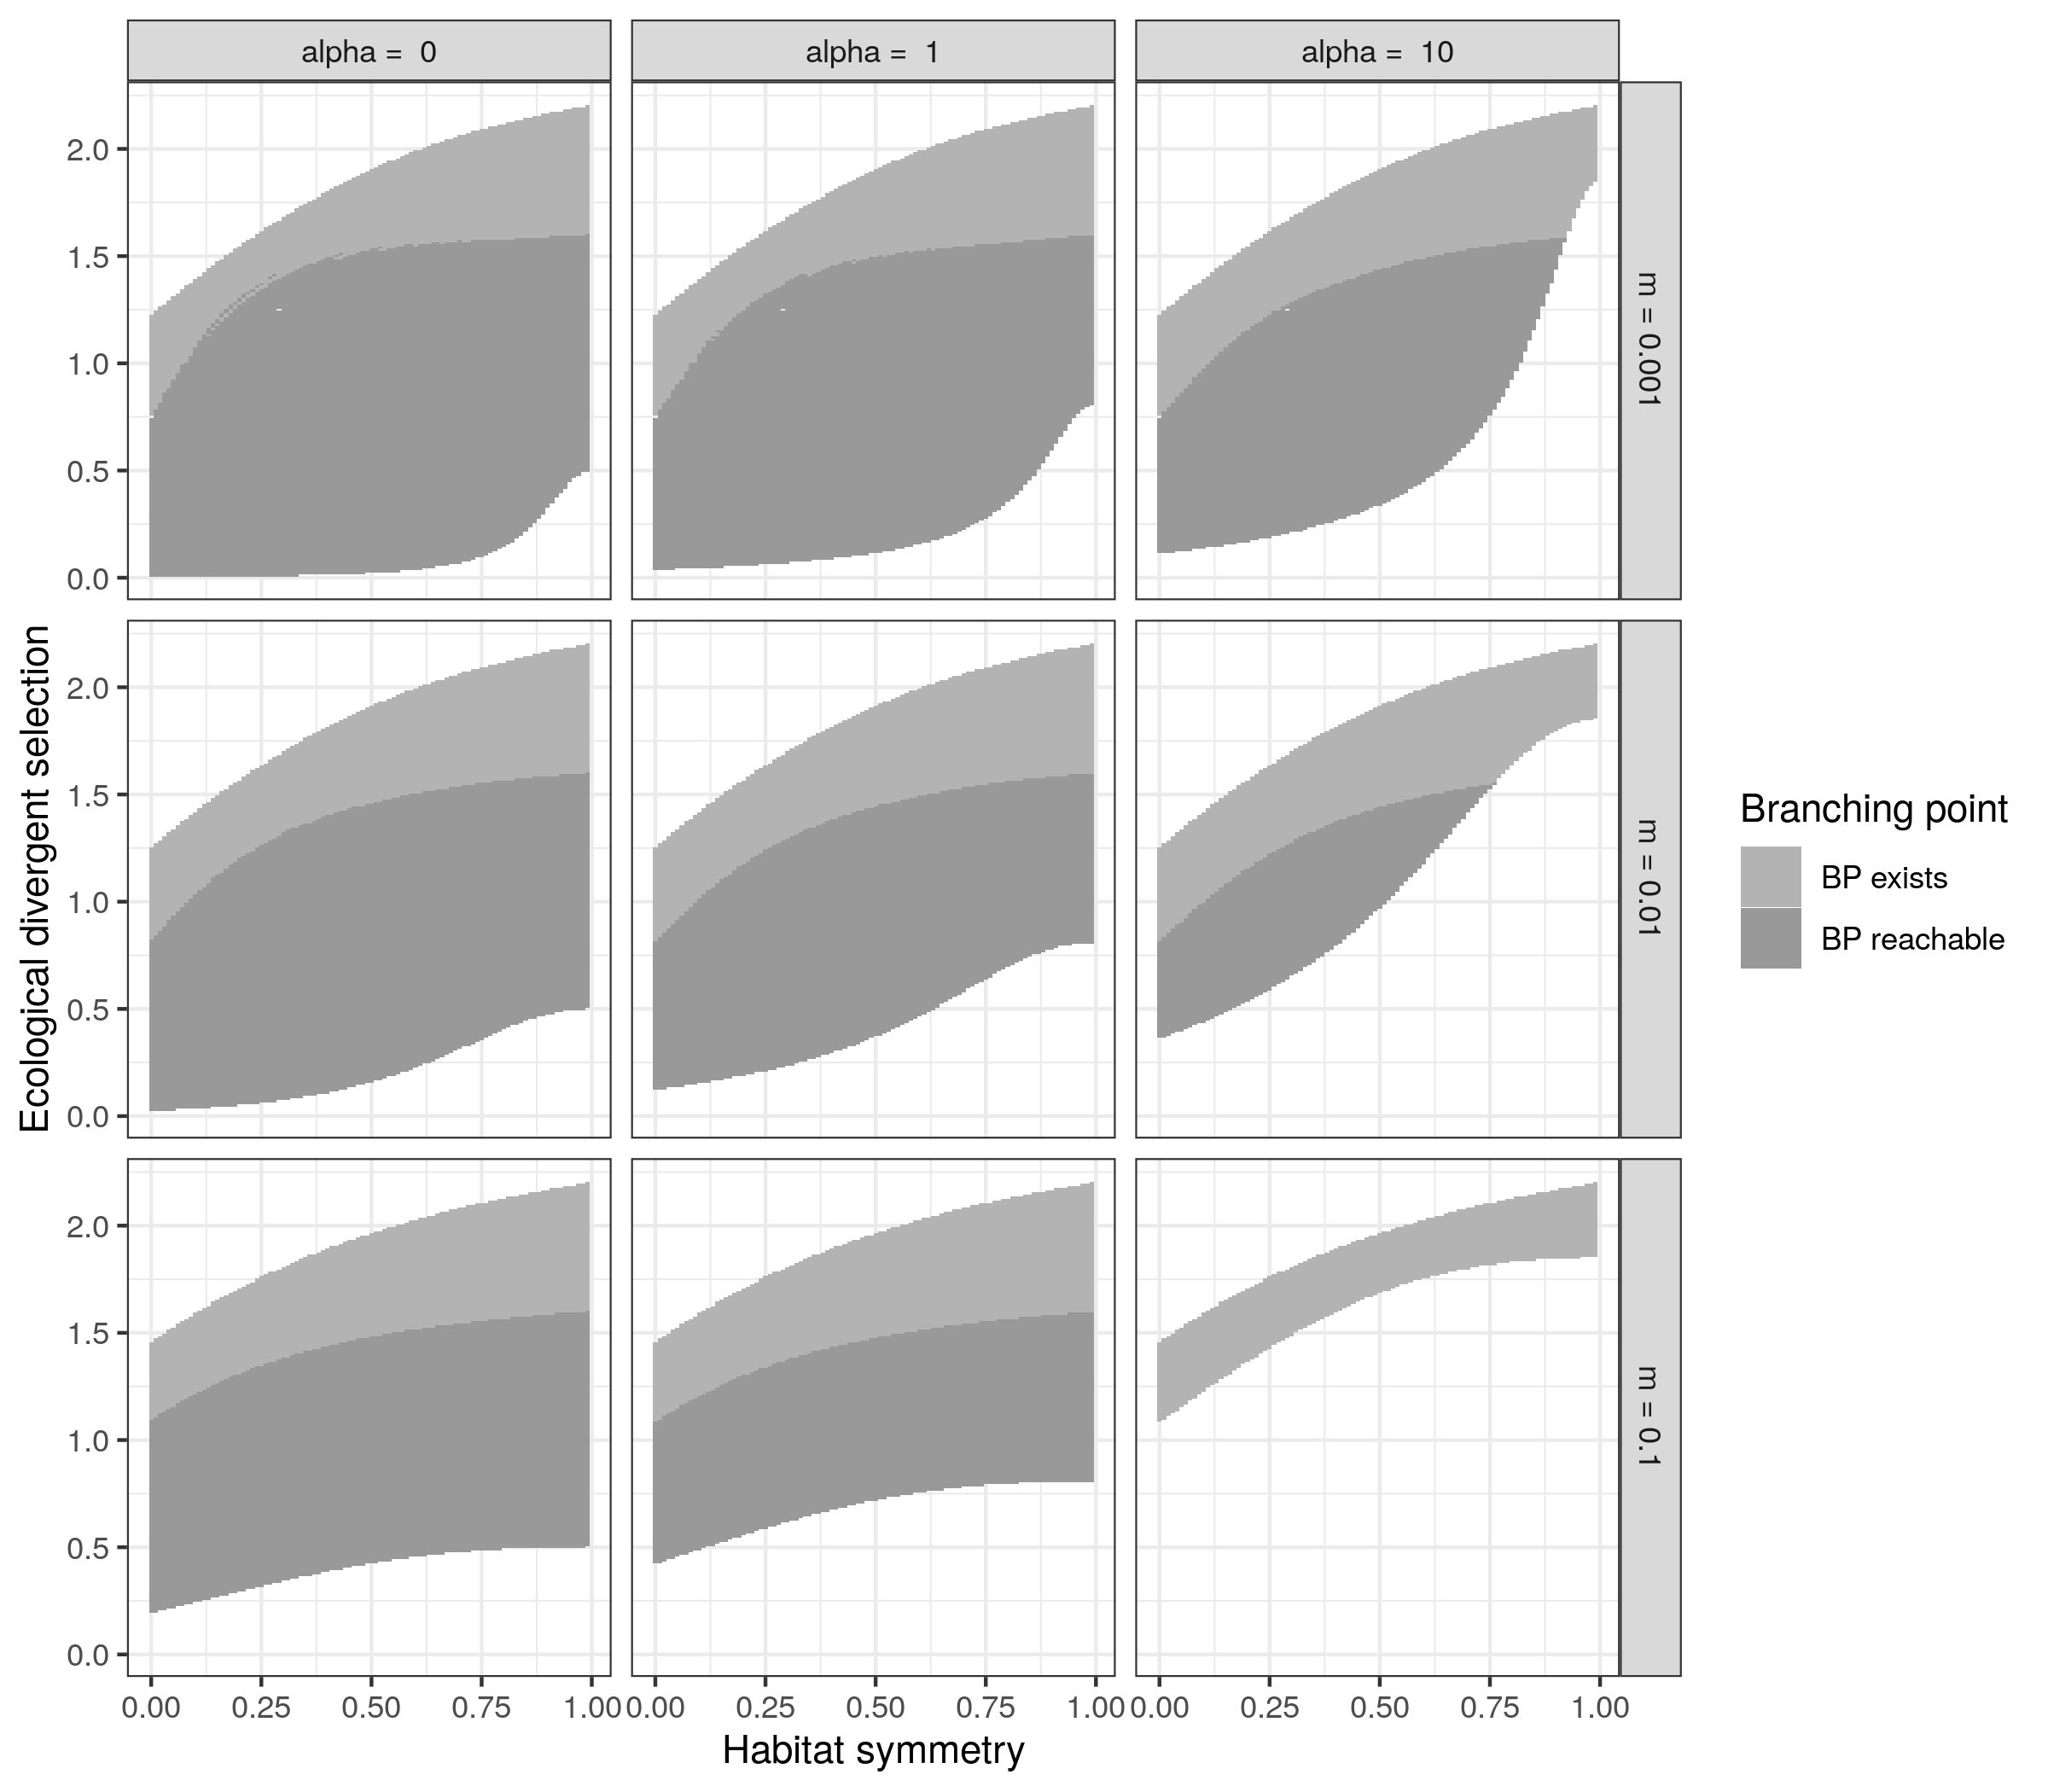
\includegraphics[width=\textwidth]{figures/branching_points_combined.png}
    \caption{Existence and attainability of a branching point through parameter space, when starting at a trait value of $x = -1$. Even if a branching point may exist, a population starting off as a specialist may not be able to reach it.}
    \label{fig:adaptive_dynamics2}
\end{figure}